\documentclass[table]{beamer}
%%\documentclass[handout]{beamer}

\mode<presentation>
{
  \definecolor{navitialight}{RGB}{126,186,200}
  \definecolor{navitiadark}{RGB}{76,102,114}

  \useoutertheme[subsection=false]{miniframes}
  %%\useoutertheme[footline=authortitle]{miniframes}
  \usecolortheme[named=navitiadark]{structure}
  %%\usecolortheme{dolphin}
  \usecolortheme{orchid}
  \useinnertheme{circles}
  \setbeamerfont{block title}{size=\normalsize}
  \setbeamercovered{transparent}

  %%% le foot pour avoir la numérotation des slides %%%
  \setbeamertemplate{footline}{%
    \leavevmode%
    \hbox{%
      \begin{beamercolorbox}[wd=.5\paperwidth,ht=2.5ex,dp=1.125ex,
        leftskip=.3cm plus1fill,rightskip=.3cm]{author in head/foot}%
        \usebeamerfont{title in head/foot}\insertshorttitle
      \end{beamercolorbox}%
      \begin{beamercolorbox}[wd=.5\paperwidth,ht=2.5ex,dp=1.125ex,
        leftskip=.3cm,rightskip=.3cm plus1fil]{title in head/foot}%
        \usebeamerfont{author in head/foot}\insertshortauthor\hfill
        \insertframenumber/\inserttotalframenumber
      \end{beamercolorbox}%
    }%
    \vskip0pt%
  }

  \setbeamercolor{palette primary}{fg=white,bg=navitiadark}
  \setbeamercolor{palette secondary}{fg=white,bg=navitialight}
  \setbeamercolor{palette tertiary}{fg=white,bg=navitiadark}
  \setbeamercolor{palette quaternary}{fg=white,bg=navitialight}
}

\mode<handout>
{
  \usepackage{pgfpages}
  \pgfpagesuselayout{4 on 1}[a4paper,border shrink=5mm,landscape]
}

\usepackage[utf8]{inputenc}
\usepackage{lmodern}
\usepackage[T1]{fontenc}
\usepackage[french,english]{babel}
\usepackage{multirow}
\usepackage{hhline}

\newcommand{\nologo}{\setbeamertemplate{logo}{}}

\newenvironment{foreignpar}[1][english]{%
    \em\selectlanguage{#1}%
}{}
\newcommand*{\foreign}[2][english]{%
    \emph{\foreignlanguage{#1}{#2}}%
}

\title{Why navitia's model doesn't fit in GTFS}

\author{Guillaume Pinot}

\institute[Kisio Digital] % (optional, but mostly needed)
{
  Kisio Digital\\
  20 rue Hector Malot\\
  75012 Paris, France}
%% - Use the \inst command only if there are several affiliations.
%% - Keep it simple, no one is interested in your street address.

\date{Transit Data Workshop 2017}
%% - Either use conference name or its abbreviation.
%% - Not really informative to the audience, more for people (including
%%   yourself) who are reading the slides online

%% If you have a file called "university-logo-filename.xxx", where xxx
%% is a graphic format that can be processed by latex or pdflatex,
%% resp., then you can add a logo as follows:
\pgfdeclareimage[width=.2\linewidth]{logo}{images/logo_nio}
\logo{\pgfuseimage{logo}\hspace{.04\linewidth}}


%% Delete this, if you do not want the table of contents to pop up at
%% the beginning of each subsection:
\AtBeginSection[]
{
  \begin{frame}<beamer>
    \frametitle{Table des matières}
    \tableofcontents[currentsection,hideothersubsections]
  \end{frame}
}
\AtBeginSubsection[]
{
  \begin{frame}<beamer>
    \frametitle{Table des matières}
    \tableofcontents[currentsection,subsectionstyle=show/shaded/hide]
  \end{frame}
}


\begin{document}

\begin{frame}
  \titlepage
\end{frame}

\begin{frame}
  \frametitle{navitia model}

  \centering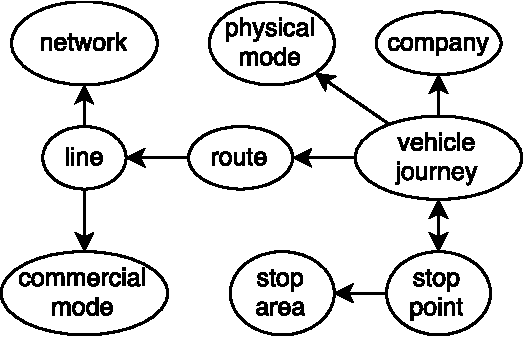
\includegraphics[width=0.9\linewidth]{images/navitia-model}
\end{frame}

\begin{frame}
  \frametitle{stops.txt: OK}

  \centering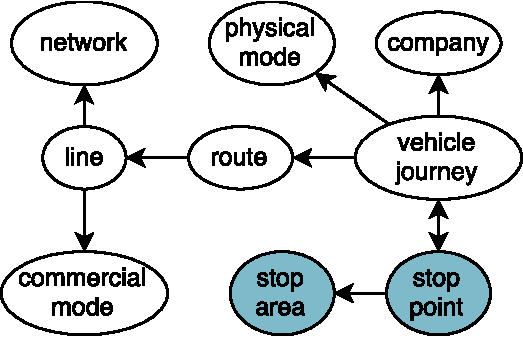
\includegraphics[width=0.9\linewidth]{images/navitia-model-stops}
\end{frame}

\begin{frame}
  \frametitle{trips.txt + stop\_times.txt + calendar.txt + ...: OK}

  \centering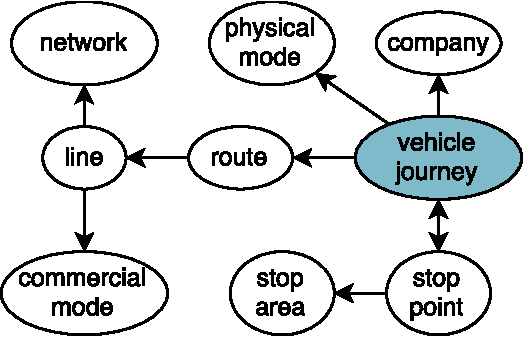
\includegraphics[width=0.9\linewidth]{images/navitia-model-trips}
\end{frame}

\begin{frame}
  \frametitle{About agency.txt}

  \centering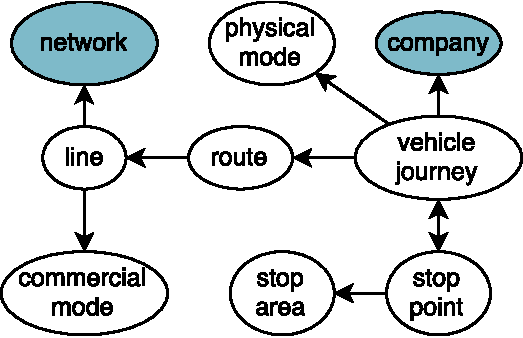
\includegraphics[width=0.9\linewidth]{images/navitia-model-agency}
\end{frame}

\begin{frame}
  \frametitle{More or less routes.route\_type}

  \centering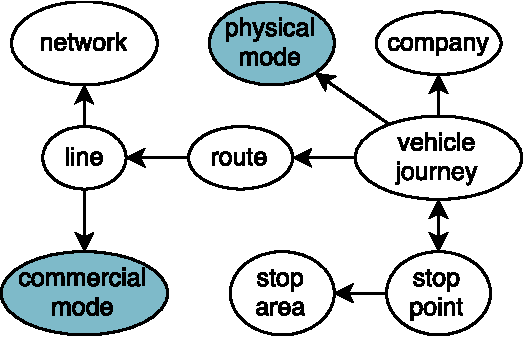
\includegraphics[width=0.9\linewidth]{images/navitia-model-route-type}
\end{frame}

\begin{frame}
  \frametitle{Something like routes.txt + trips.direction\_id}

  \centering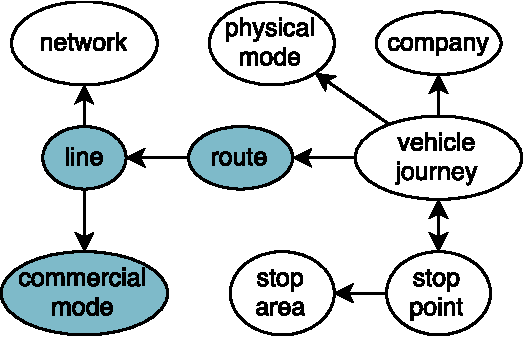
\includegraphics[width=0.9\linewidth]{images/navitia-model-routes}
\end{frame}

\begin{frame}
  \frametitle{BusWay 4}
  
  \begin{columns}
    \begin{column}{0.6\linewidth}
      navitia:
      \begin{itemize}
      \item commercial mode: BusWay
      \item line.code: 4
      \item routes:
        \begin{itemize}
        \item route1.name: Foch Cathédrale
        \item route2.name: Porte de Vertou
        \end{itemize}
      \end{itemize}

      GTFS:
      \begin{itemize}
      \item route.code: BusWay 4
      \item trip.direction\_id:
        \begin{itemize}
        \item 0
        \item 1
        \end{itemize}
      \end{itemize}
    \end{column}
    \begin{column}{0.3\linewidth}
      \centering
      
\includegraphics[width=0.5\linewidth]{images/busway-logo}

      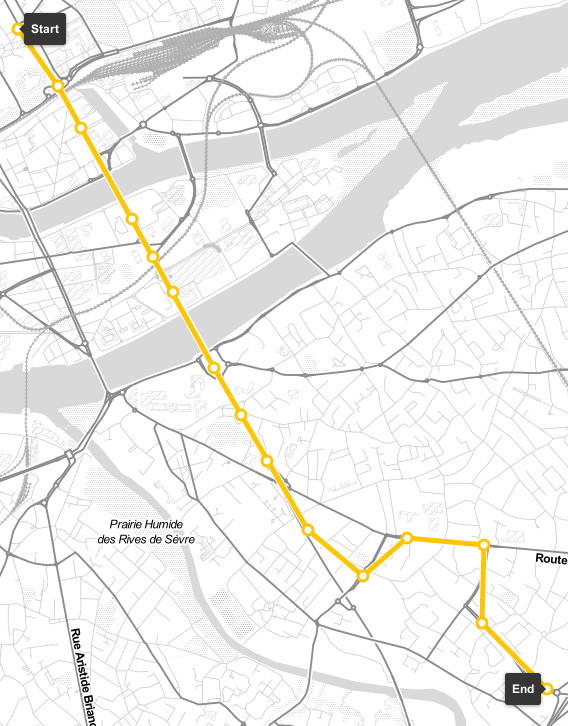
\includegraphics[width=\linewidth]{images/busway-map}      
    \end{column}
  \end{columns}
\end{frame}

\begin{frame}
  \frametitle{RER A}
  
  \begin{columns}
    \begin{column}{0.7\linewidth}
      \scriptsize

      navitia:
      \begin{itemize}
      \item commercial mode: RER
      \item line.code: A
      \item routes:
        \begin{itemize}
          \scriptsize
        \item route1.name: Cergy-Le-Haut
        \item route2.name: Poissy
        \item route3.name: Saint-Germain-en-Laye
        \item route4.name: Marne-la-Vallée
        \item route5.name: Boissy-Saint-Léger
        \end{itemize}
      \end{itemize}

      GTFS (2 directions each):
      \begin{itemize}
      \item route.code: RER A Cergy-le-Haut -- Marne-la-Vallée
      \item route.code: RER A Cergy-le-Haut -- Boissy-Saint-Léger
      \item route.code: RER A Poissy -- Marne-la-Vallée
      \item route.code: RER A Poissy -- Boissy-Saint-Léger
      \item route.code: RER A Saint-Germain-en-Laye -- Marne-la-Vallée
      \item route.code: RER A Boissy-Saint-Léger -- Boissy-Saint-Léger
      \end{itemize}
    \end{column}
    \begin{column}{0.3\linewidth}
      \centering
      
\includegraphics[width=0.5\linewidth]{images/rer-a-logo}

      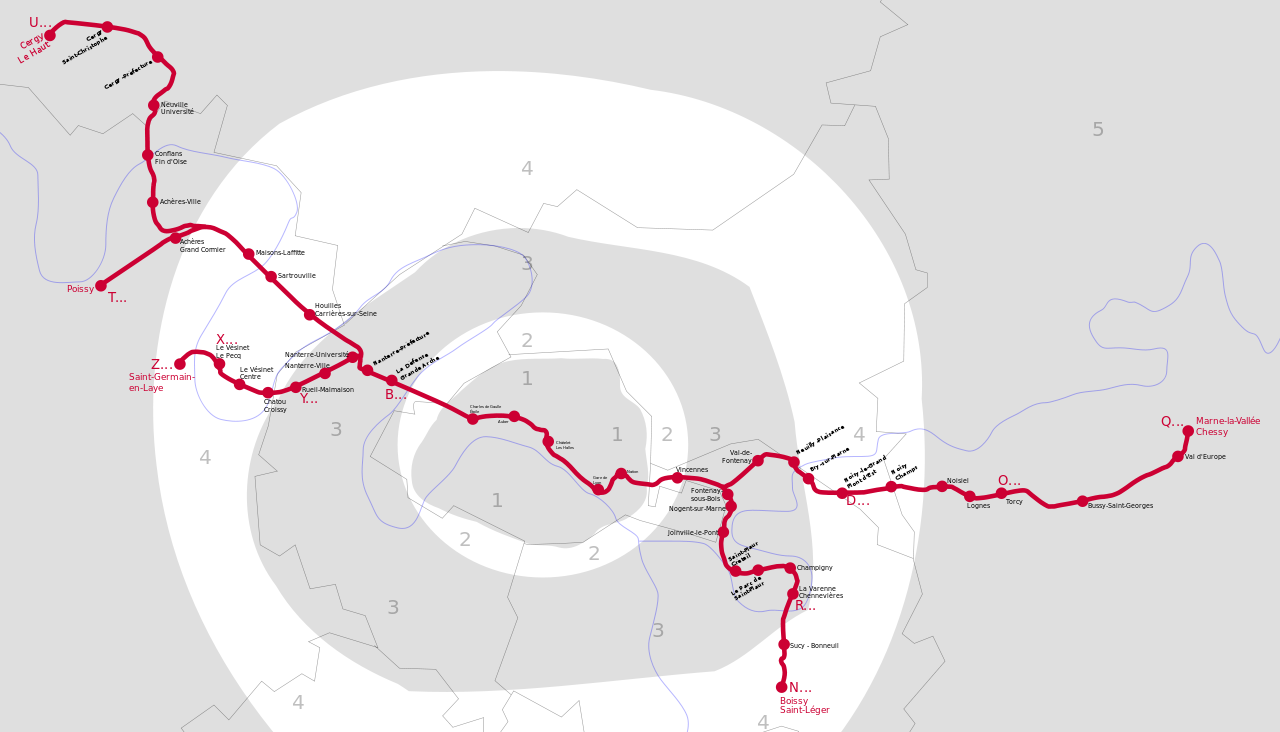
\includegraphics[width=\linewidth]{images/rer-a-map}      
    \end{column}
  \end{columns}
\end{frame}

\begin{frame}
  \frametitle{RER C}

  \begin{columns}
    \begin{column}{0.2\linewidth}
      
\includegraphics[width=\linewidth]{images/rer-c-logo}      
    \end{column}
    \begin{column}{0.3\linewidth}
      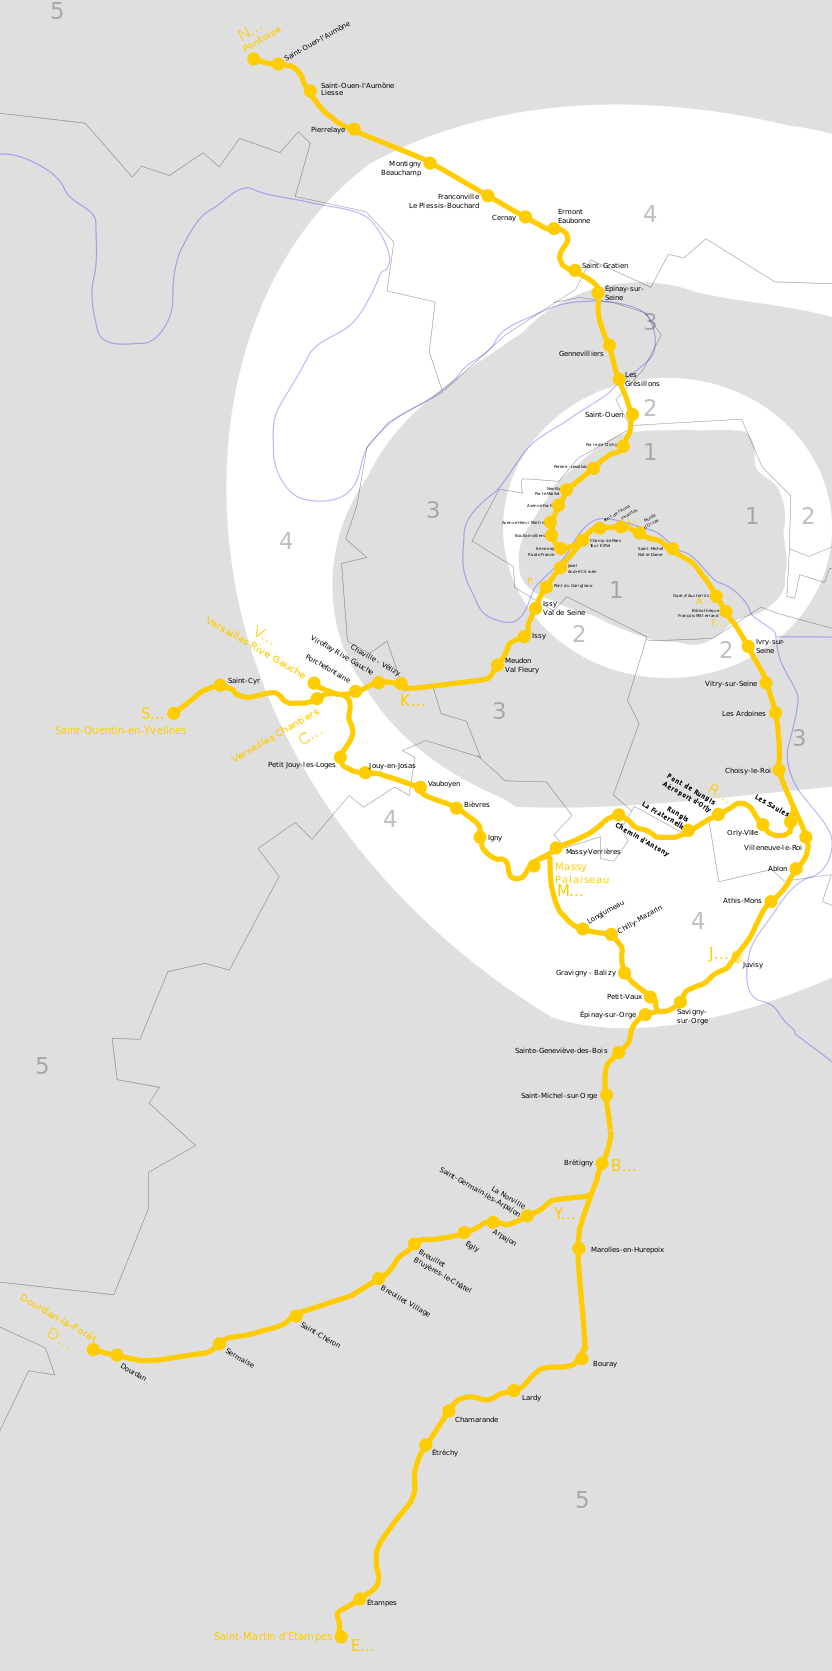
\includegraphics[width=\linewidth]{images/rer-c-map}      
    \end{column}
  \end{columns}
\end{frame}

\begin{frame}
  \titlepage
\end{frame}

\end{document}
